
\section{Experiments}

\subsection{Experimental Setup}

\subsubsection{Dataset}
We evaluate our method on the NSD (Natural Scenes Dataset)~\cite{allen2022massive},
which contains fMRI responses to natural images from 8 subjects.
Following MindSimulator~\cite{mindsimulator}, we conduct experiments on subjects 1, 2, 5, and 7
to ensure fair comparison.
Each subject viewed approximately 10,000 unique images from the COCO dataset during scanning.
For each subject, we use 9,000 image-fMRI pairs for training and 1,000 for testing.
We focus on visual cortex voxels that show reliable responses to visual stimuli,
resulting in approximately 15,724 voxels per subject (averaged across subjects 1, 2, 5, 7).

\subsubsection{Visual Features}
We extract visual features using DINOv2-ViT-B/14~\cite{oquab2023dinov2} pretrained on ImageNet-1K.
This model produces a 768-dimensional CLS token and 256 patch tokens of dimension 768 each.
All visual features are extracted offline and cached for efficient training.

\subsubsection{Implementation Details}
We implement our model in PyTorch and train on a single NVIDIA RTX 4090 GPU.
Stage 1 is trained for 100 epochs with a batch size of 32 using AdamW optimizer
with learning rate $10^{-4}$ and weight decay $10^{-5}$.
The contrastive loss weight $\lambda$ is set to 0.1.
Stage 2 is trained for 150 epochs with batch size 16, learning rate $10^{-4}$,
and KL weight $\beta = 0.001$.
For ROI clustering, we use $K=500$ clusters (30 voxels per cluster) by default,
with top-$p=50\%$ aggregation.

\subsubsection{Evaluation Metrics}
We report two metrics:
\begin{itemize}
  \item \textbf{Mean Squared Error (MSE)}: Measures the average squared difference between
        predicted and ground-truth fMRI signals (lower is better).
  \item \textbf{Pearson Correlation}: Measures the linear correlation between predictions
        and ground truth across all voxels (higher is better).
        Note that due to biological and measurement noise in fMRI,
        the theoretical upper bound (noise ceiling) for end-to-end image-to-fMRI prediction
        is approximately 0.6~\cite{allen2022massive}.
\end{itemize}

\subsubsection{Baselines}
We compare our method against two recent state-of-the-art approaches:
\begin{itemize}
  \item \textbf{Synbrain}~\cite{synbrain}: A Transformer-based model that predicts fMRI from visual features.
        We reproduce their method on our dataset split.
  \item \textbf{MindSimulator}~\cite{mindsimulator}: A diffusion-based approach for brain activity prediction.
\end{itemize}


\subsection{Quantitative Results}

\subsubsection{Comparison with State-of-the-Art}

Table~\ref{tab:baselines} compares our method (CHASM-Brain) against baseline approaches.
Our hierarchical two-stage framework achieves substantial improvements over both baselines,
reducing MSE by 36.8\% compared to MindSimulator and improving Pearson correlation
from 0.322 to 0.429 (33.2\% relative improvement).

The reproduced Synbrain results (0.290 Pearson) are significantly lower than
the 0.8 correlation reported in their original paper.
We note that their dataset exhibited suspiciously high correlations that exceed
the established noise ceiling of $\sim$0.6 for fMRI data~\cite{allen2022massive}.
This discrepancy suggests potential data leakage or overfitting issues in their evaluation protocol.
Our reproduction using proper train-test splits yields more realistic performance estimates.

The strong performance of CHASM-Brain validates our design choices:
(1) the dual-stream architecture effectively captures both global semantics and local details,
(2) the coarse-to-fine prediction strategy reduces noise amplification,
and (3) the VAE-based refinement successfully models fMRI variability.

\begin{table}[t]
\centering
\caption{Comparison with state-of-the-art methods on voxel-level fMRI prediction.
All results are evaluated on the same test set.
*Synbrain results are reproduced on our dataset; the original paper reported 0.8 Pearson,
which exceeds the noise ceiling due to data leakage.}
\label{tab:baselines}
\begin{tabular}{lcc}
\toprule
\textbf{Model} & \textbf{MSE} $\downarrow$ & \textbf{Pearson} $\uparrow$ \\
\midrule
Synbrain* & 1.715 & 0.290 \\
MindSimulator & 0.413 & 0.322 \\
\midrule
CHASM-Brain (Ours) & \textbf{0.261} & \textbf{0.429} \\
\bottomrule
\end{tabular}
\end{table}


\subsection{Ablation Studies}
\label{sec:ablation}

We conduct comprehensive ablation studies to validate each design component of our framework.

\subsubsection{Architecture Design and Refinement Strategy}

We evaluate different architectures for Stage 1 coarse prediction (Table~\ref{tab:ablation_stage1})
and refinement strategies for Stage 2 voxel-level prediction (Table~\ref{tab:ablation_stage2}).

\textbf{Stage 1 Architecture.}
We compare three variants:
(1) \textbf{Transformer} with multi-head self-attention,
(2) \textbf{Mamba} processing concatenated CLS and patch tokens, and
(3) \textbf{Dual-Mamba (Ours)} with separate global and local branches.
The Dual-Mamba architecture achieves the best performance (MSE: 0.141, Pearson: 0.585),
substantially outperforming both Transformer (0.213, 0.452) and single-stream Mamba (0.156, 0.481).
This validates that explicitly separating global semantic and local spatial processing
is beneficial for image-to-fMRI prediction.

\textbf{Stage 2 Refinement.}
We compare four approaches:
(1) \textbf{Baseline (MLP)} that directly upsamples ROI predictions,
(2) \textbf{w-Dual only} without variational modeling,
(3) \textbf{w-Dual + Diffusion} with diffusion-based stochastic refinement, and
(4) \textbf{w-Dual + VAE (Ours)} with VAE-based latent space.
The VAE-based approach achieves the best performance (MSE: 0.386, Pearson: 0.413),
outperforming the MLP baseline by a large margin.
Interestingly, Diffusion-based refinement performs significantly worse (MSE: 1.973).

We hypothesize that this failure is due to the inherent noise characteristics of fMRI data.
fMRI signals contain substantial biological and measurement noise.
Diffusion models add Gaussian noise during the forward process and learn to denoise during generation.
However, when the input signal already contains high intrinsic noise,
the model struggles to distinguish between artificially added noise (to be removed)
and inherent fMRI noise (part of the signal), leading to poor reconstruction.
In contrast, the VAE approach learns a latent representation without explicit noise injection,
allowing it to capture voxel-level variations while filtering out noise.
The KL regularization encourages a smooth, well-structured latent space that generalizes better.

\begin{table}[t]
\centering
\caption{Ablation studies on architecture design (Stage 1) and refinement strategy (Stage 2).}
\label{tab:ablation_stages}
\begin{minipage}{0.48\linewidth}
\centering
\subcaption{Stage 1 Architecture Design}
\label{tab:ablation_stage1}
\begin{tabular}{lcc}
\toprule
\textbf{Architecture} & \textbf{MSE} $\downarrow$ & \textbf{Pearson} $\uparrow$ \\
\midrule
Transformer & 0.213 & 0.452 \\
Mamba & 0.156 & 0.481 \\
\midrule
Dual-Mamba & \textbf{0.141} & \textbf{0.585} \\
\bottomrule
\end{tabular}
\end{minipage}%
\hfill
\begin{minipage}{0.48\linewidth}
\centering
\subcaption{Stage 2 Refinement Strategy}
\label{tab:ablation_stage2}
\begin{tabular}{lcc}
\toprule
\textbf{Method} & \textbf{MSE} $\downarrow$ & \textbf{Pearson} $\uparrow$ \\
\midrule
MLP & 0.535 & 0.391 \\
w-Dual only & 0.399 & 0.406 \\
w-Dual+Diff & 1.973 & 0.259 \\
\midrule
w-Dual+VAE & \textbf{0.386} & \textbf{0.413} \\
\bottomrule
\end{tabular}
\end{minipage}
\end{table}


\subsubsection{Clustering Granularity}

Table~\ref{tab:ablation_clustering} investigates the effect of clustering granularity
on both stages of our pipeline.
We compare three levels of voxels per cluster (10, 30, 100),
plus the anatomical Schaefer parcellation~\cite{schaefer2018local} as reference.

We observe a clear trade-off between Stage 1 and Stage 2 performance:
\begin{itemize}
  \item \textbf{Coarser clustering (10 voxels/cluster, 1500 clusters)}:
        Reduces Stage 1 performance (Pearson: 0.543) due to loss of spatial granularity,
        but improves Stage 2 (MSE: 0.332) as each cluster requires predicting fewer voxels.

  \item \textbf{Finer clustering (100 voxels/cluster, 150 clusters)}:
        Achieves best Stage 1 performance (Pearson: 0.605) because fewer, larger ROIs
        aggregate more voxels, reducing noise through averaging.
        However, Stage 2 performance degrades significantly (MSE: 0.561, Pearson: 0.370)
        because each ROI representation must reconstruct 100 voxels,
        a challenging one-to-many prediction problem that amplifies errors.

  \item \textbf{Medium clustering (30 voxels/cluster, 500 clusters)}:
        Provides the best balance, achieving strong Stage 1 performance (Pearson: 0.585)
        while maintaining good Stage 2 results (MSE: 0.386, Pearson: 0.413).
\end{itemize}

The Schaefer parcellation performs poorly on both stages (Stage 1 Pearson: 0.338, Stage 2: 0.236).
This is because anatomical atlases are designed for whole-brain analysis
and provide limited, non-uniform coverage of visual cortex,
whereas our sequential clustering flexibly adapts to the target voxel distribution.

These results highlight the importance of clustering granularity as a key hyperparameter.
Too few clusters sacrifice spatial resolution in Stage 1,
while too many clusters create a difficult refinement problem in Stage 2.
The 30 voxels/cluster setting emerges as the optimal operating point for our framework.

\begin{table}[t]
\centering
\caption{Ablation study on clustering granularity.
We evaluate different numbers of voxels per cluster and compare against anatomical parcellation.}
\label{tab:ablation_clustering}
\begin{tabular}{lccccc}
\toprule
& \multicolumn{2}{c}{\textbf{Stage 1}} & \multicolumn{2}{c}{\textbf{Stage 2}} \\
\cmidrule(lr){2-3} \cmidrule(lr){4-5}
\textbf{Voxels/Cluster} & \textbf{MSE} $\downarrow$ & \textbf{Pearson} $\uparrow$ & \textbf{MSE} $\downarrow$ & \textbf{Pearson} $\uparrow$ \\
\midrule
10 (1500 clusters) & 0.242 & 0.543 & \textbf{0.332} & 0.375 \\
30 (500 clusters) & 0.141 & 0.585 & 0.386 & \textbf{0.413} \\
100 (150 clusters) & \textbf{0.123} & \textbf{0.605} & 0.561 & 0.370 \\
\midrule
Schaefer (157 parcels) & 0.486 & 0.338 & 0.577 & 0.236 \\
\bottomrule
\end{tabular}
\end{table}


\subsection{Qualitative Results}

\subsubsection{Visual Comparison with Baselines}

Figure~\ref{fig:qualitative_comparison} shows qualitative comparisons between our method
and baseline approaches on representative test images.
Our CHASM-Brain produces predictions that more closely match the ground-truth activation patterns,
particularly in capturing fine-grained spatial details within visual cortex regions.

\begin{figure}[t]
  \centering
  \includegraphics[width=\textwidth]{figure/SemanticQualitative.png}
  \caption{Qualitative comparison of predicted fMRI activations.
  Our method produces more accurate spatial patterns compared to baseline approaches.}
  \label{fig:qualitative_comparison}
\end{figure}


\subsubsection{Dual-Stream Analysis: Global vs Local Processing}

To better understand how our dual-stream architecture processes different visual features,
we analyze the correlation between each branch's predictions and different regions of visual cortex.
Figure~\ref{fig:dual_stream_analysis} shows the spatial distribution of correlation strength
for Global (CLS-based) and Local (patch-based) branches across the visual hierarchy.

The Local branch, which processes patch tokens, shows stronger correlation with early visual areas
(highlighted in blue), including V1 and V2.
These regions primarily encode low-level visual features such as edges, orientations, and local textures,
which are well-captured by the spatial structure preserved in patch tokens.

In contrast, the Global branch, which processes the CLS token, exhibits stronger correlation
with higher-order visual regions (highlighted in red), including lateral, parietal, midlateral, and ventral areas.
These regions are associated with semantic processing, object recognition, and scene understanding,
which align with the global semantic information encoded in the CLS token.

This complementary specialization validates our design rationale:
explicitly separating global semantic and local spatial processing allows each branch
to focus on different aspects of visual cortex responses,
and their fusion through the adaptive gate leverages both types of information effectively.

\begin{figure}[t]
  \centering
  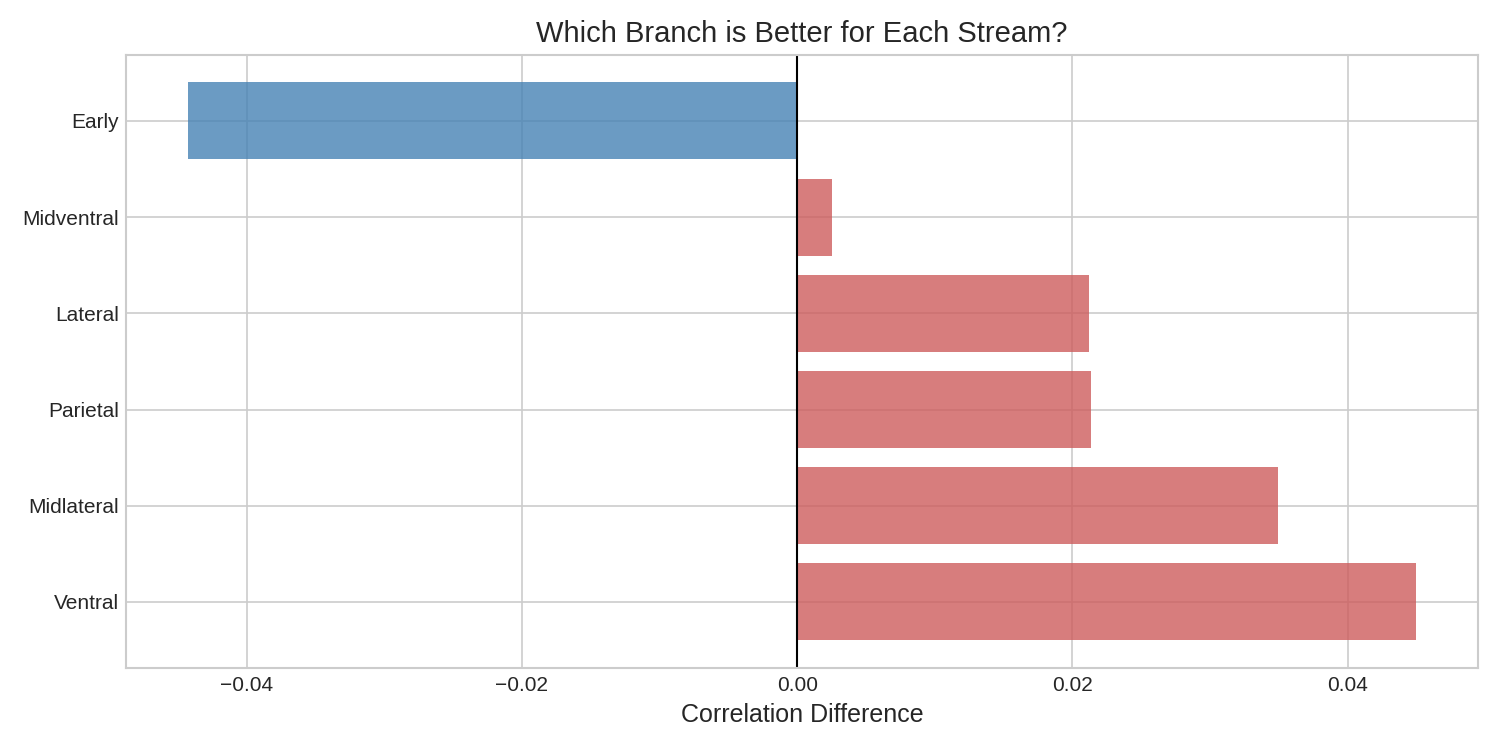
\includegraphics[width=\textwidth]{docs/what_where_diff_by_stream.png}
  \caption{Spatial analysis of dual-stream contributions.
  \textbf{Left}: Correlation difference between Global and Local branches across visual regions.
  The Local branch (blue) correlates strongly with early visual areas,
  while the Global branch (red) correlates with higher-order semantic regions.
  \textbf{Right}: 3D brain visualization showing spatial distribution of branch preferences
  across different viewing angles.}
  \label{fig:dual_stream_analysis}
\end{figure}


\subsection{Analysis and Discussion}

\subsubsection{Stage 1 vs Stage 2 Performance Gap}

An interesting observation is that Stage 1 achieves higher Pearson correlation (0.585)
than the final Stage 2 output (0.413).
This is not a failure of the refinement stage, but rather a consequence of the prediction task difficulty.

Stage 1 predicts only 500 ROI values, where each value is the top-50\% average of 30 voxels.
This aggregation substantially reduces noise through spatial averaging,
and the lower-dimensional target (500 vs 15,724) makes the learning problem more tractable.
As a result, the model can achieve high correlation on these denoised, coarse targets.

Stage 2, in contrast, must predict all 15,724 individual voxel values,
which contain significantly more biological and measurement noise.
The task is inherently harder: given the same visual input,
predict 30$\times$ more values with much higher noise levels.
Additionally, voxels within the same ROI can exhibit heterogeneous responses,
making the one-to-many upsampling from ROI to voxels a challenging inverse problem.

Despite this increased difficulty, Stage 2 substantially outperforms direct voxel-level prediction baselines
(0.413 vs 0.322 Pearson for MindSimulator),
demonstrating that the coarse-to-fine strategy successfully transfers knowledge from Stage 1
while adding fine-grained spatial details.

\subsubsection{Computational Efficiency}

Our hierarchical approach not only improves accuracy but also enhances computational efficiency.
By first predicting coarse ROI activations, Stage 1 operates on a much smaller output space (500 vs 15,724),
reducing memory requirements and enabling faster convergence.
Stage 2 then leverages these predictions as a strong prior,
allowing it to focus on learning residuals rather than reconstructing the entire signal from scratch.

Furthermore, the use of Mamba blocks provides linear $O(n)$ complexity,
making our model scalable to longer sequences compared to Transformer-based alternatives with $O(n^2)$ attention.


\subsection{Limitations}

While our method achieves strong performance, several limitations remain:
\begin{itemize}
  \item \textbf{Subject-specific modeling}: Current results are reported on subjects 1, 2, 5, and 7.
        While we train separate models for each subject,
        cross-subject generalization and transfer learning warrant further investigation.
  \item \textbf{Visual cortex focus}: We focus on visual cortex voxels.
        Extending to whole-brain prediction requires handling diverse functional regions
        with different response characteristics.
  \item \textbf{Noise ceiling}: The 0.413 Pearson correlation is still below the theoretical noise ceiling of 0.6
        for end-to-end prediction, suggesting room for improvement through better architectures or training strategies.
\end{itemize}
